%%%%%%%%%%%%%%%%%%%%%%%%%%%%%%%%%%%%%%%%%%%%%%%%%%%%%%%%%%%%%%%%%%%%%%%%%%%%%
%
% This is a template ATLAS Paper that contains suggestions and hints on
% how to get your note in a form that minimizes the amount of work
% needed to get it approved by the collaboration - assuming that the
% physics is OK!
%
%%%%%%%%%%%%%%%%%%%%%%%%%%%%%%%%%%%%%%%%%%%%%%%%%%%%%%%%%%%%%%%%%%%%%%%%%%%%%%

\documentclass[11pt,a4paper]{atlasnote}
\graphicspath{{figures/}}
\usepackage{atlasphysics}
\usepackage{subfigure}
\usepackage{mathrsfs}

%%%%%%%%%%%%%%%%%%%%%%%%%%%%%%%%%%%%%%%%%%%%%%%%%%%%%%%%%%%%%%%%%%%%%%%%%%%%%%
% Preamble
%%%%%%%%%%%%%%%%%%%%%%%%%%%%%%%%%%%%%%%%%%%%%%%%%%%%%%%%%%%%%%%%%%%%%%%%%%%%%%

\title{A template for ATLAS papers}
%\author{The ATLAS Collaboration}
%\draftversion{1.0}

\abstracttext{
  
  This is a template ATLAS paper. It contains the structure, style
  files and hints on how to produce a paper for which a minimum amount
  of time is necessary to spend on typographic details. This template
  can be found on the web pages of the ATLAS Publication
  Committee. You can find some \LaTeX{} technical detail about the
  template in the Appendix of this paper.
  A couple of remarks about the paper front page:
  \begin{itemize}

  \item {\bf Title:} it should be concise, clear and descriptive, and
    should include the word ``ATLAS''.

  \item {\bf Author list:} it will be provided by the Authorship
    Committee, and will be made available on their website. On the
    front page, you should name ``The ATLAS Collaboration'' as
    author.

  \item {\bf Abstract:} it should also be clear, descriptive, and
    concise. It should ideally be one paragraph long, and certainly no
    
  \end{itemize}
}

%%%%%%%%%%%%%%%%%%%%%%%%%%%%%%%%%%%%%%%%%%%%%%%%%%%%%%%%%%%%%%%%%%%%%%%%%%%%%%%
% This is where the document really begins
%%%%%%%%%%%%%%%%%%%%%%%%%%%%%%%%%%%%%%%%%%%%%%%%%%%%%%%%%%%%%%%%%%%%%%%%%%%%%%%

% Shorthand for \phantom to use in tables
\newcommand{\pho}{\phantom{0}}
\newcommand{\bslash}{\ensuremath{\backslash}}
\newcommand{\BibTeX}{{\sc Bib\TeX}}

\begin{document}

\tableofcontents
\clearpage

\section{Introduction}

The introduction should be fairly brief, not more than one page.
State the measurement being made, motivate its importance
experimentally and theoretically. Include a summary of what is known
to date about this measurement. Give a brief outline for the rest of
the paper.

Your first action before embarking on writing a paper should be to
read the ATLAS Publication Policy~\cite{publication_policy}, available
from the web pages of the Publication Committee. Chapter 3 of this
document details the refereeing and approval procedures that you will
need to follow; chapter 4 gives information on the style.

At some point during writing of an ATLAS paper, you should decide what
journal it will be submitted to.  Please keep in mind that each
journal makes specific demands on length and style.  Most journals use
regular capitalization for titles (i.e. capitalize the first word and
all proper nouns, e.g. ``The search for large extra dimensions''). The
notable exception is Physical Review Letters, which capitalizes the
first word and all other important words, e.g. ``The Search for Large
Extra Dimensions''.

The \LaTeX{} file and Postscript versions of this template can be
found on the web pages of the ATLAS Publication Committee. Example
macros for figures can be found there as well.  Comments and/or
suggestions on improvements to this template are very welcome and
should be given to the publication committee.

This paper template has been tested using \LaTeX{}2e.  You should get
this version automatically. If you have problems check which \LaTeX{}
version you are running.

\section{Theory}

Give here a brief explanation of the theory relevant for this paper,
with proper referencing. Use, for example,
\verb|\cite{Glashow:1961tr,Weinberg:1967tq,sm_salam}| to cite the
Standard Model~\cite{Glashow:1961tr,Weinberg:1967tq,sm_salam}.

Define important quantities that will be used later.  State how the
measurement of interest is actually performed, and how parameters are
extracted from the data.  If quantities are extracted with a fit to
the data, describe the fit procedure. If the explanation needs to be a
bit longer, a separate section may be appropriate.

The {\tt atlasphysics.sty} style file contains a set of particles,
reactions, etc. that may be useful. For example, the missing-$E_T$
symbol (\met{}) is defined there. Appendix~\ref{app:AtlasPhysicsSty}
contains a list of some of the commands in {\tt atlasphysics.sty}.

\section{Experimental setup}

The Publication Committee will provide a standard text giving a brief
description of the ATLAS detector, and the appropriate references.  If
necessary for your analysis, describe a subdetector in more detail.

Describe the data set: when were the data taken, under what special
circumstances (if any), and what was the integrated luminosity.

\section{Monte Carlo}

Any Monte Carlo programs used must be clearly stated with full version
number. A brief description of the program is useful but not necessary
unless a less well known program is used.  Any corrections or special
parameter settings must be clearly explained.  The statistics should
be given if the amount used results in a non-negligible uncertainty.

\section{Event selection}

List the trigger and offline selection criteria, give the obtained
statistics.

\subsection{Tables}

All tables appearing in the paper must be mentioned in the text. The
tables should appear in the same order as mentioned in the text. Do
not abbreviate the word ``Table''. Capitalize the first word of any
row or column heading. Label all rows/columns, including units if
appropriate. Units are given in brackets, e.g. ``Energy [\gev]''.
Horizontal and vertical lines should be used as necessary to make the
table entries clear. 
The table caption appears below the table.  
Any symbols/variables used in the table must be defined in the
caption.  Always use labels to refer to tables and figures. Note that
the label must be included in the body of the caption.

If table entries include uncertainties, the entries should be aligned
on the ``$\pm$'' sign. Numbers look best when aligned on the decimal
point. Otherwise, column entries should be left-aligned.
Table~\ref{tab:example1} shows the use of $\pm$ as the intercolumn
character for alignment. An alternative, as shown in
Table~\ref{tab:example2}, is to use \verb+\phantom+ to put in extra
space equal to the width of a number if you have different numbers of
decimal places in the table.


\begin{table}
  \begin{center}
    \begin{tabular}{lr@{$\pm$}lr}
      \hline \hline
      Category      & \multicolumn{2}{c}{$\mu$}&\multicolumn{1}{c}{e}\\ 
      \hline
      $\btol $       &     65.2 & 0.4\%   &  79.3\% \\
      $\btoctol$     &      7.8 & 0.3\%   &   5.4\% \\
      Total          &     73.0 & 0.2\%   &   9.1\% \\ 
      \hline \hline
    \end{tabular}
  \caption[Monte Carlo purities in the single lepton sample]{% Monte
    Carlo estimates of the fraction of each process in the single
    lepton data sample. This table uses {\tt $\pm$} as the intercolumn
    separator.}
  \label{tab:example1}
  \end{center}
\end{table}


\begin{table}
  \begin{center}
    \begin{tabular}{lcc}
      \hline \hline
      Category      & \multicolumn{1}{c}{$\mu$}&\multicolumn{1}{c}{e}\\ 
      \hline
      $\btol $       & $    65.2 \pm 0.4\%$   &     79.3\% \\
      $\btoctol$     & $\pho 7.8 \pm 0.3\%$   & \pho 5.4\% \\
      Total          & $    73.0 \pm 0.2\%$   & \pho 9.1\% \\ 
      \hline \hline
    \end{tabular}
  \caption{Monte Carlo estimates of the fraction of each process in
    the single lepton data sample. This table uses {\tt \bslash
    phantom}.}
  \label{tab:example2}
  \end{center}
\end{table}

%
%%%%%%%%%%%%%%%%%%%%%%%%%%%%%%%%%%%%%%%%%%%%%%%%%%%%%%%%%%%%%%%%%%%%%%%%%%%%%%%
% Data characteristics
%%%%%%%%%%%%%%%%%%%%%%%%%%%%%%%%%%%%%%%%%%%%%%%%%%%%%%%%%%%%%%%%%%%%%%%%%%%%%%%
%
\section{Data characteristics}

Discuss here the characteristics of the data, in terms of
primary quantities and backgrounds.

\subsection{Figures}

The Publication Committee has a root macro to create figures in
ATLAS style, it can be found on the PubComm web pages.
Use this style consistently throughout the paper.
An example figure can be seen in Figure~\ref{fig:example}. 

\begin{figure}
  \centering
  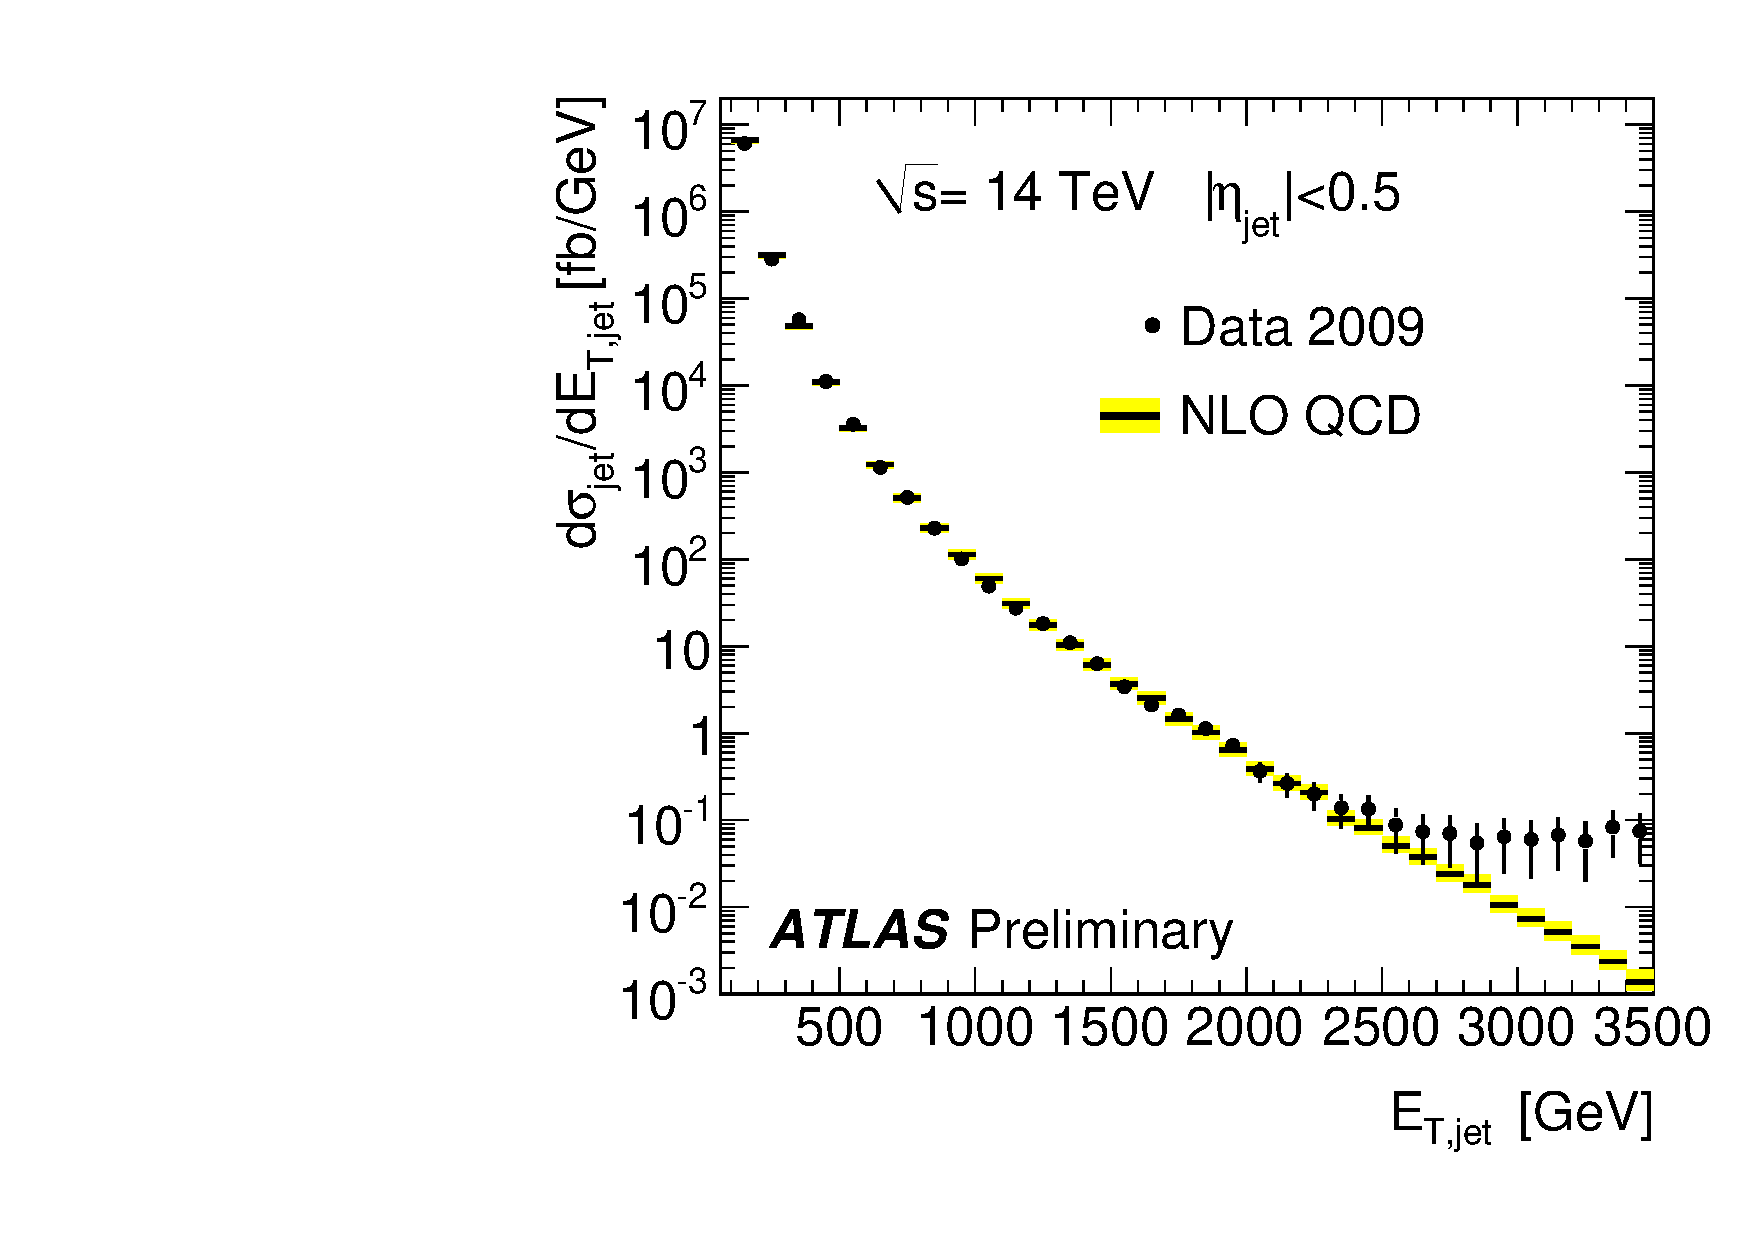
\includegraphics[width=\columnwidth]{AtlasExample}
  \caption{An example ATLAS figure.}
  \label{fig:example}
\end{figure}

Figures should be always made available in both {\tt eps} and {\tt
  png} format. Additionally, a {\tt pdf} version of the plots can be
useful in case \verb|pdflatex| is used to produce a publication.
%Colour versions are appropriate for talks, and black-and-white
%versions are necessary for the publication itself.

All figures appearing in the paper must be mentioned in the text.
The figures should appear in the same order as mentioned in the text.
At the beginning of a sentence, use the full word ``Figure''.
Within a sentence, the abbreviation ``Fig.'' may be used.
If a figure appears in two or more parts, refer to it as
``Fig. 1(a)'' and ``Fig. 1(b)''. Both ``(a)'' and ``(b)'' should
appear in the text, in the figure, and in the caption.
The word ``ATLAS'' (or ``ATLAS Preliminary'', if appropriate) should
appear prominently somewhere in the figure. This becomes important when
the figure is copied and shown out of context. If appropriate, it
is useful to include information about the luminosity corresponding
to a figure.

All axes must be labeled, including units (i.e. ``Energy [\gev]'').
The vertical axis units should specify the bin width, unless
arbitrarily normalized. A legend box explaining all plotting symbols
must appear somewhere in the figure.

The caption should be placed below the figure.  All lines, all
plotting symbols, and all variables used in the figure must be defined
in the caption. Do not refer to any characteristic that is not
distinguishable in black-and-white.  If relevant, the normalization
method of the plot should be specified.

A figure with subfigures can be made as shown in the example of
Figure~\ref{fig:subfigexample}.

\begin{figure}
  \centering
  \subfigure[One subfigure example]{
    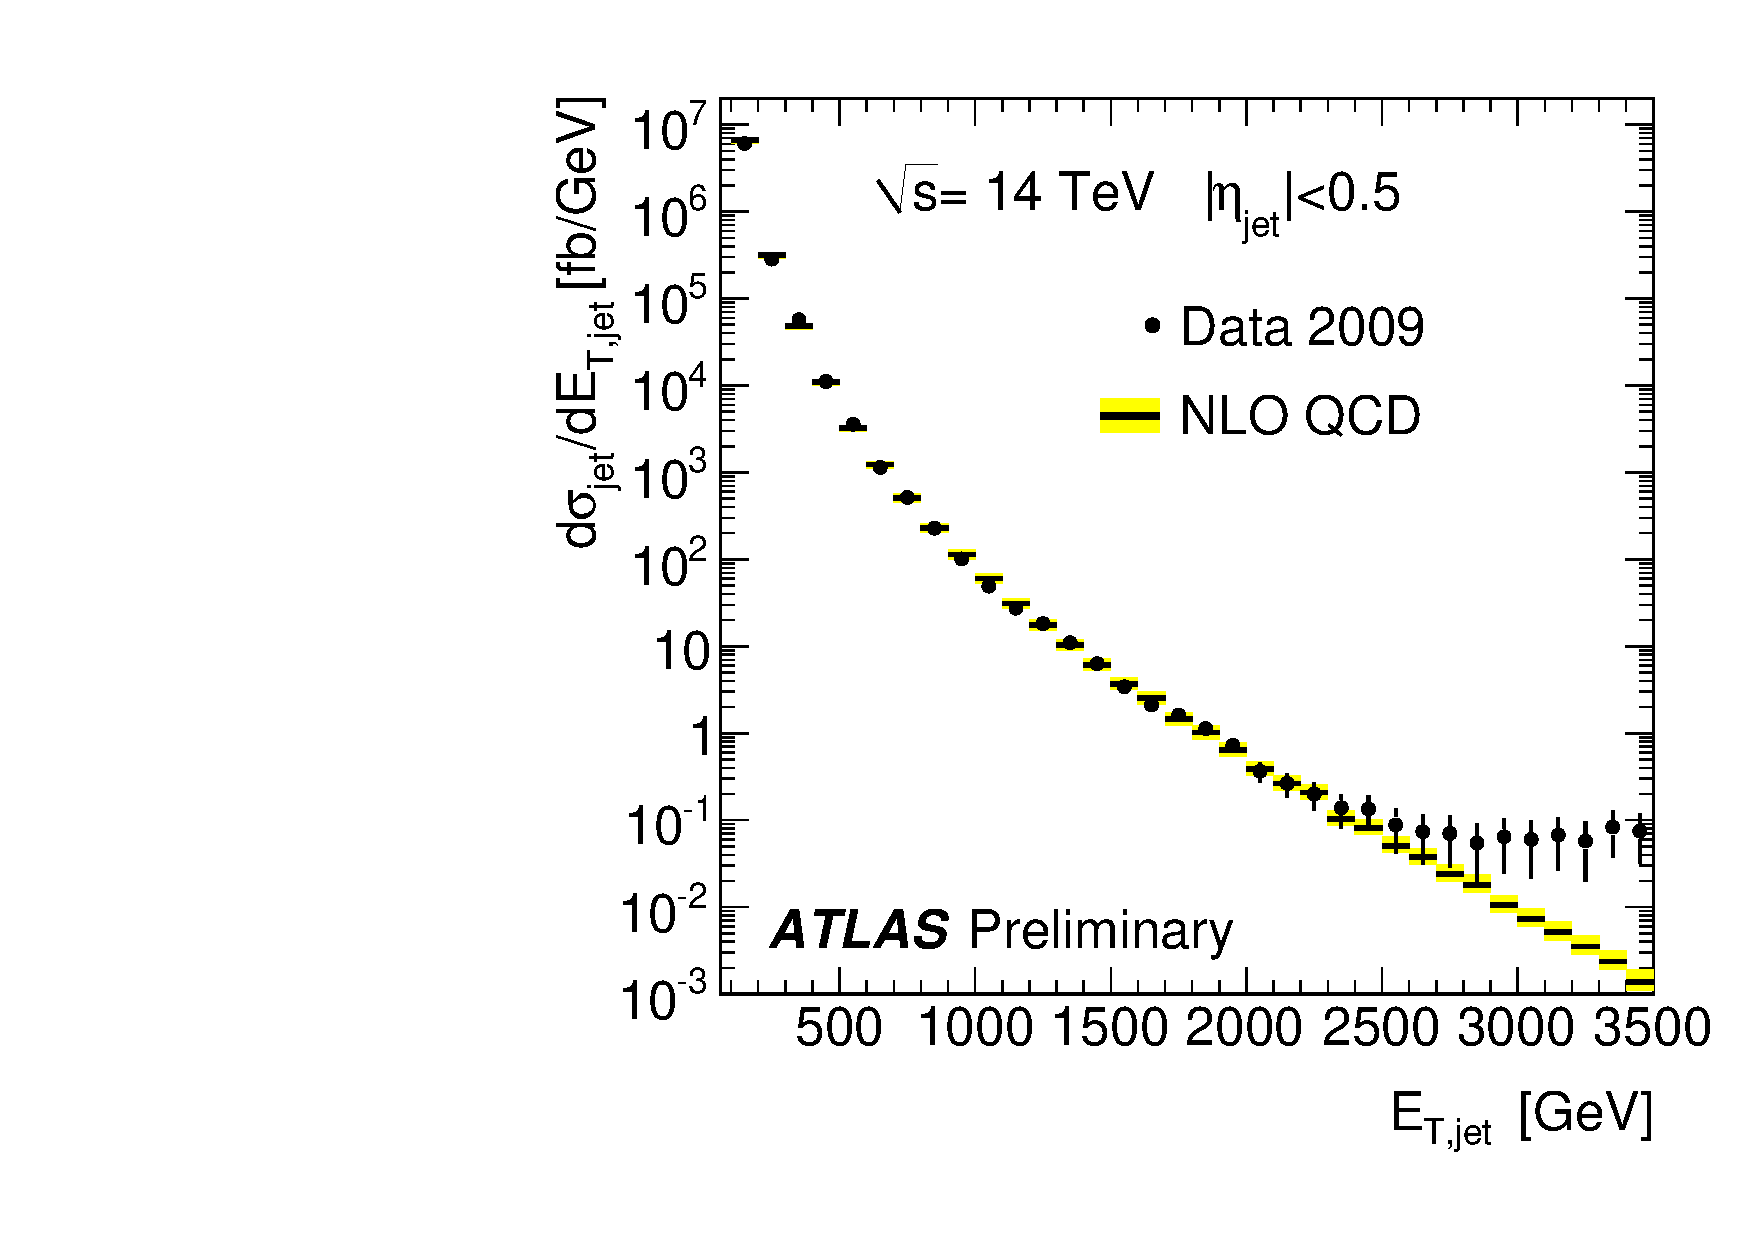
\includegraphics[width=0.55\textwidth]{AtlasExample}
    \label{fig:SubfigureExample1}
  }
  \subfigure[Another subfigure example]{
    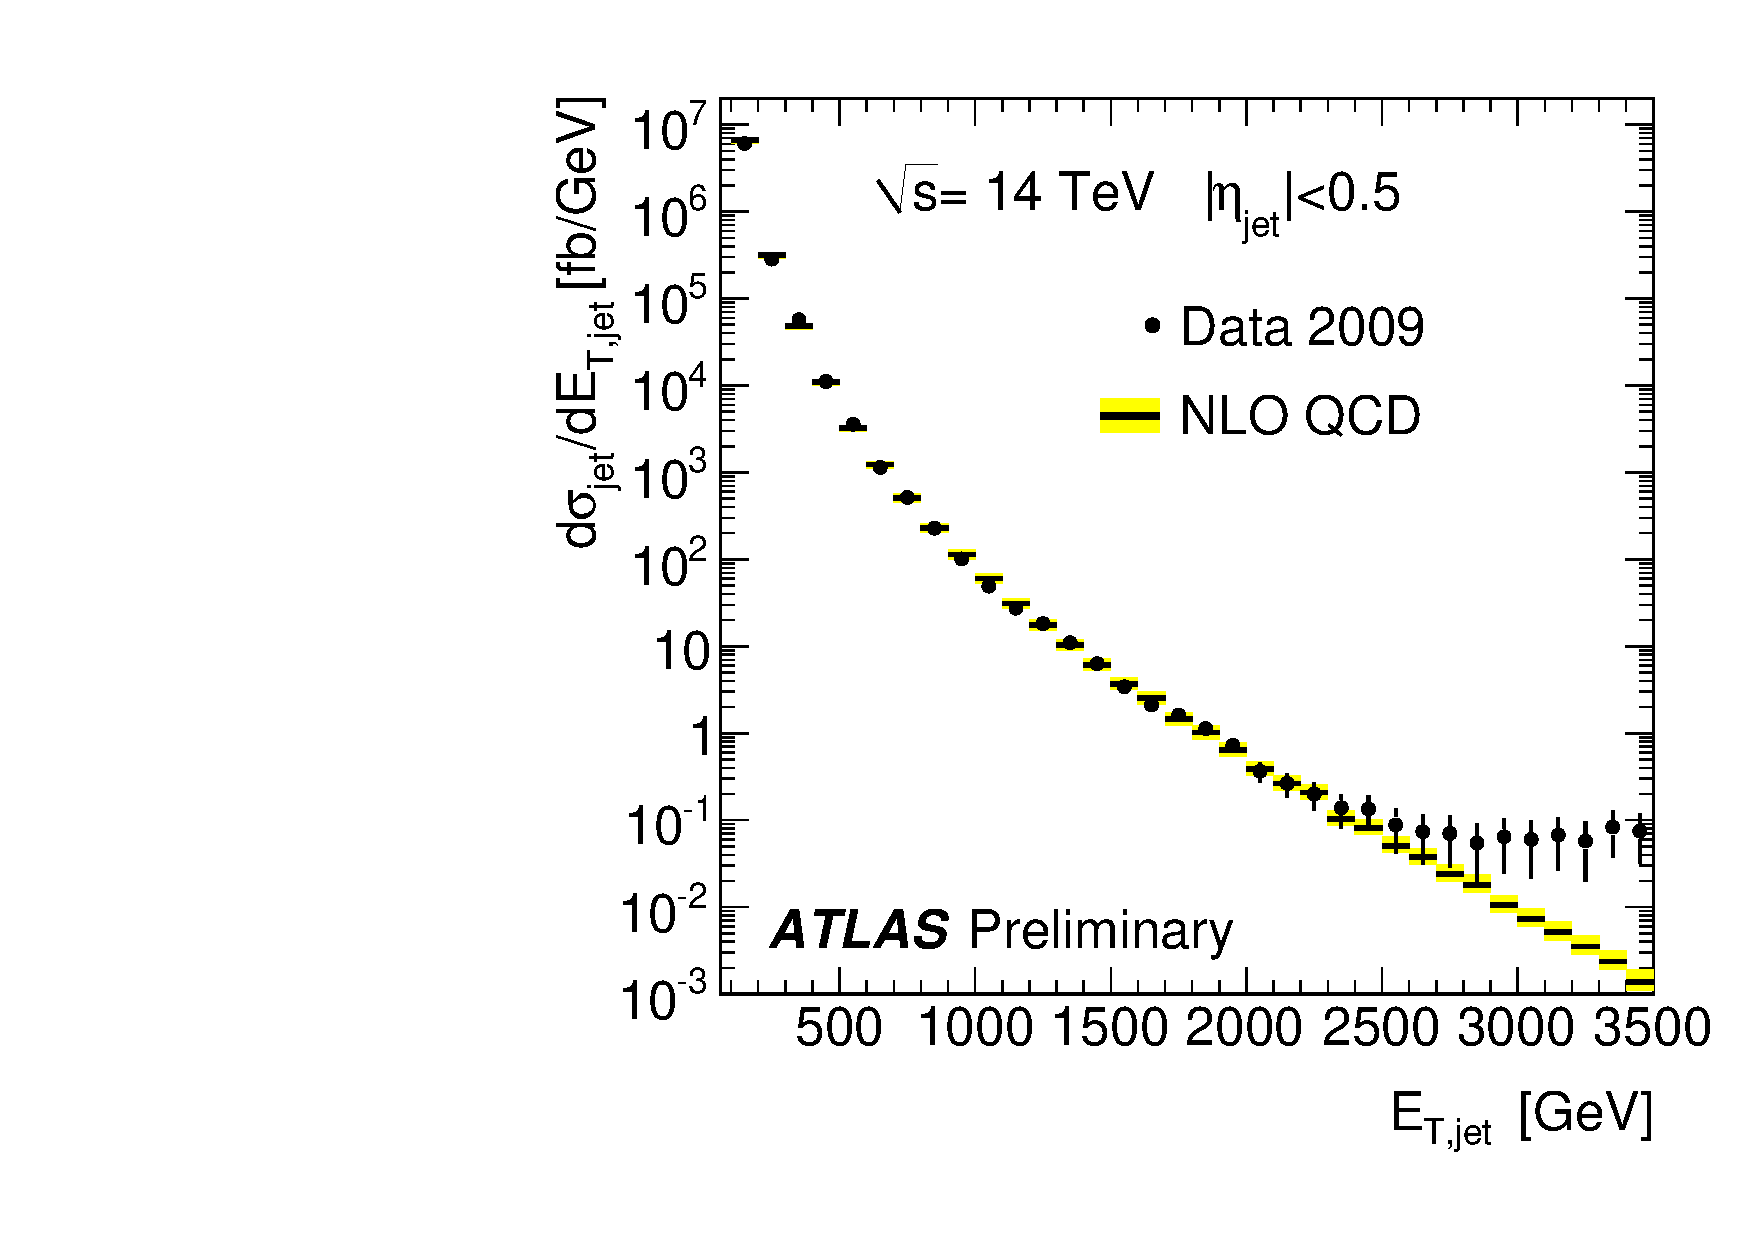
\includegraphics[width= 0.55\textwidth]{AtlasExample}
    \label{fig:SubfigureExample2}
  }
  \caption{Subfigure example (\ref{fig:SubfigureExample1}) and
    (\ref{fig:SubfigureExample2}).}
  \label{fig:subfigexample}
\end{figure}

%
%%%%%%%%%%%%%%%%%%%%%%%%%%%%%%%%%%%%%%%%%%%%%%%%%%%%%%%%%%%%%%%%%%%%%%%%%%%%%%%
% Systematic uncertainties
%%%%%%%%%%%%%%%%%%%%%%%%%%%%%%%%%%%%%%%%%%%%%%%%%%%%%%%%%%%%%%%%%%%%%%%%%%%%%%%
%
\section{Systematic uncertainties}

Give a detailed list of systematic uncertainties, the method
by which they were obtained, and a justification of the resulting
values.
%
Use ``systematic uncertainty'' instead of ``systematic errors''.
The latter sounds as if you have made a mistake systematically.

%
%%%%%%%%%%%%%%%%%%%%%%%%%%%%%%%%%%%%%%%%%%%%%%%%%%%%%%%%%%%%%%%%%%%%%%%%%%%%%%%
% Results
%%%%%%%%%%%%%%%%%%%%%%%%%%%%%%%%%%%%%%%%%%%%%%%%%%%%%%%%%%%%%%%%%%%%%%%%%%%%%%%
%
\section{Results}

State the results without interpretations.

%
%%%%%%%%%%%%%%%%%%%%%%%%%%%%%%%%%%%%%%%%%%%%%%%%%%%%%%%%%%%%%%%%%%%%%%%%%%%%%%%
% Discussion
%%%%%%%%%%%%%%%%%%%%%%%%%%%%%%%%%%%%%%%%%%%%%%%%%%%%%%%%%%%%%%%%%%%%%%%%%%%%%%%
%
\section{Discussion}

Put the results into the context of the theory or a model.
%
If the results lead to exclusion plots, make sure that it is clear 
which region on the plot is excluded.

%
%%%%%%%%%%%%%%%%%%%%%%%%%%%%%%%%%%%%%%%%%%%%%%%%%%%%%%%%%%%%%%%%%%%%%%%%%%%%%%%
% Summary and conclusion
%%%%%%%%%%%%%%%%%%%%%%%%%%%%%%%%%%%%%%%%%%%%%%%%%%%%%%%%%%%%%%%%%%%%%%%%%%%%%%%
%
\section{Summary and conclusion}

Reiterate the main points of the paper and the primary results and
conclusions.

Note that many readers look mostly at the title, abstract and
conclusion. The conclusion should be interesting enough to
make them want to read the whole paper.
It is not good style to just repeat the abstract.

If your paper is short and only has one result quoted at the end of
the paper, then you should consider whether conclusions are
necessary. 

Try not to end your conclusions with a sentence such as
``All the results in this paper are in good agreement with the
Standard Model, the current world average and recent
measurements by other experiments''. This might lead a referee
(internal or external) to wonder why it is worth publishing this
paper!

%
%%%%%%%%%%%%%%%%%%%%%%%%%%%%%%%%%%%%%%%%%%%%%%%%%%%%%%%%%%%%%%%%%%%%%%%%%%%%%%%
% Acknowledgements
%%%%%%%%%%%%%%%%%%%%%%%%%%%%%%%%%%%%%%%%%%%%%%%%%%%%%%%%%%%%%%%%%%%%%%%%%%%%%%%
%
\section{Acknowledgements}

A standard template for the acknowledgements is available on the
web pages of the Publication Committee.
See reference~\cite{publication_policy} for the URL. 

%
%%%%%%%%%%%%%%%%%%%%%%%%%%%%%%%%%%%%%%%%%%%%%%%%%%%%%%%%%%%%%%%%%%%%%%%%%%%%%%%
% Rules for referencing
%%%%%%%%%%%%%%%%%%%%%%%%%%%%%%%%%%%%%%%%%%%%%%%%%%%%%%%%%%%%%%%%%%%%%%%%%%%%%%%
%
\section{Rules for referencing}

Use \BibTeX{} for the references. See Appendix~\ref{app:References}
for an explanation.

Only cite permanent, publicly available, or ATLAS approved references.
Private references, not available to the general public, should be
avoided. Caution should be used when referring to ATLAS notes.
Only reference approved notes. Do not reference COM or INT notes,
as these are not available outside ATLAS.

Whenever possible, cite the article's journal rather than its
preprint number. If desired, the hep-ex number can be given in
addition. Always double check references when copying them from
another source.

Referencing styles are journal-dependent. See the ATLAS Publication
Policy document for more information.

%%%%%%%%%%%%%%%%%%%%%%%%%%%%%%%%%%%%%%%%%%%%%%%%%%%%%%%%%%%%%%%%%%%%%%%%%%%%%%%
% Bibliography
%%%%%%%%%%%%%%%%%%%%%%%%%%%%%%%%%%%%%%%%%%%%%%%%%%%%%%%%%%%%%%%%%%%%%%%%%%%%%%

\bibliographystyle{atlasnote}
\bibliography{instructions}

%%%%%%%%%%%%%%%%%%%%%%%%%%%%%%%%%%%%%%%%%%%%%%%%%%%%%%%%%%%%%%%%%%%%%%%%%%%%%%%
% Technical Aspects
%%%%%%%%%%%%%%%%%%%%%%%%%%%%%%%%%%%%%%%%%%%%%%%%%%%%%%%%%%%%%%%%%%%%%%%%%%%%%%%

\newpage
\appendix
\part*{Appendices}
\addcontentsline{toc}{part}{Appendices}

Use the Appendices to include all the technical details of your work
that are relevant for the ATLAS Collaboration only (e.g. datases
details, software release used). The Appendices can be removed from
an ATLAS Internal Note becoming an ATLAS Public Note.

Use the following commands to start the Appendices section:
\begin{verbatim}
   \newpage
   \appendix
   \part*{Appendices}
   \addcontentsline{toc}{part}{Appendices}
\end{verbatim}

\section{The {\tt atlasnote} class}
\label{app:AtlasNoteCls}

This paper has been typeset using the {\tt atlasnote.cls} class, that
implement the ATLAS template can be used for papers, preprints,
notes. The {\tt atlasnote} class is available on web pages of the
Publication Committee, as well as this instruction paper and the
related files.

{\tt atlasnote.cls} derives from the standard \LaTeX{} {article.cls}
class, thus all the usual commands and options you would have used
with {\tt article} will work with it. For instance, this paper has
been produced using this very simple preamble:

\begin{verbatim}
  \documentclass[11pt,a4paper]{atlasnote}
  \graphicspath{{figures/}}
  \usepackage{atlasphysics}
  \usepackage{subfigure}
\end{verbatim}

\subsection{Dependencies}

The {\tt atlasnote} class depends on these packages, which presence in
your system is required:
\begin{itemize}
  \item {\tt graphicx}
  \item {\tt mathptmx}
  \item {\tt lineno}
\end{itemize}
The first two are all usually already installed in any modern \LaTeX{}
installation, while the latter is part of the {\tt ednotes} package
bundle and is direclty provided with this package; {\tt atlasnote} was
tested on a CERN {\tt lxplus} node and worked out of the box. The {\tt
  atlasnote} class works both with \LaTeX{} and pdf\LaTeX{}.

If you wish to use the {\tt atlascover} package with the {\tt
  atlasnote} class, load the latest version of the package in your
system, and invoke it using the {\tt coverpage} option of the class:
\begin{verbatim}
  \documentclass[11pt,a4paper,coverpage]{atlasnote}
\end{verbatim}
instead of the the usual {\tt usepackage} command: this will ensure
that the cover page is produced before the note title page.

\subsection{Custom commands}

The {\tt atlasnote} class implements some custom commands, mainly
used to typeset the frontpage content:

\begin{itemize}

  \item {\verb|\title{<Title>}|} typesets the paper title. If not
    given, a dummy \emph{Title goes here} title will be produced.

  \item {\verb|\author{<Author>}|} typesets the paper author. If not
    explicitly given, \emph{The ATLAS Collaborations} will be used by
    default. Note that the \verb|\author{}| command is pretty limited
    in case you want to display multiple author names and multiple
    affiliations. For this use case the \verb|authblk.sty| package is
    provided; this is a typical example of its use:
    \begin{verbatim}
\usepackage{authblk}
\renewcommand\Authands{, } % avoid ``. and'' for last author
\renewcommand\Affilfont{\itshape\small} % affiliation formatting

\author[a]{First Author}
\author[a]{Second Author}
\author[b]{Third Author}

\affil[a]{One Institution}
\affil[b]{Another Institution}
    \end{verbatim}

  \item {\verb|\abstracttext{<The abstract text>}|} typesets the
    abstract in the front page.

  \item {\verb|\date{<Date>}|} typesets the paper date. If not
    explicitly given, the current date (\verb|\today|) will be used.

  \item {\verb|\draftversion{<Draft Version>}|} displays the draft
    version on the front page, a DRAFT banner on all the other page
    headings, and add line numbers to all text to easy commenting abd
    reviewing. Can be omitted.

  \item {\verb|\journal{<Journal Name>}|} displays the phrase \emph{to
    be submitted to Journal Name} at the bottom of the front page. Can
    be omitted.

  \item {\verb|\skipbeforetitle{<lenght>}|} sets the distance between
    the title page header and the note title. The default value should
    be fine for most notes, but in case you have a long list of
    authors or a lenghtly abstract you can use this command to buy
    some extra space. Note that \verb|<lenght>| can also be negative
    (use it at your own risk!).

\end{itemize}

\noindent {\tt emptynote.tex} contains a basic skeleton that can be
used to start typing a new note using the {\tt atlasnote} class. All
the custom commands described above are used in this example file, in
order to demonstrate their use.

\section{Bibliography}
\label{app:References}

We recomments to use \BibTeX{} for the references. Although it often
appears harder to use at the beginning, it means that the number of
typos should be reduced significantly and the format of the references
will be correct, without you having to worry about formatting it. In
addition the order of the references is automatically correct.

A file with the extension {\tt .bib} (in this example: {\tt
instruction.bib}) should contain all the references. This file may
also contain references that you do not use, so it may act like a
library of references. The typical comilation cycle when using
\BibTeX{} looks like the following:
%
\begin{verbatim}
  (pdf)latex instructions
  bibtex instructions
  (pdf)latex instructions
  (pdf)latex instructions
\end{verbatim}
%
\BibTeX{} will create a file with the extension {\tt .bbl}, which will
contain the actual references used, and \LaTeX{} will then take care
to include them in your paper. Note that only after the third run of
\LaTeX{} will all references be correct. Unless you change a reference
you do not have to do the {\tt bibtex} step again.

A \BibTeX{} style file ({\tt atlasnote.bst}) is provided with the
ATLAS template. you can use it in your text source file like in the
following:
%
\begin{verbatim}
  \bibliographystyle{atlasnote}
  \bibliography{instructions}
\end{verbatim}
%


\section{Miscellaneous \LaTeX{} tips}
\label{app:LatexTips}

\subsection{Graphics}

Use the {\tt graphicx} package \cite{} to include your plots and
figure. The use of older packages like {\tt espfig} is deprecated.
Since the {\tt graphicx} package is required by the {\tt atlasnote}
class, it is automatically loaded when using it, and there is no need
to explicitly included it in the document preamble.

Always include your graphics file without metioning the file
extension. Fior inctance, if you want to include the {\tt figure.eps}
file, you should use a sysntax like this:
\begin{verbatim}
  \includegraphics[width=\textwidth]{figure}
\end{verbatim}
This will allow to compile your document using either \LaTeX{} or
pdf\LaTeX{} without changing your source file: you can in fact have
both {\tt figure.eps} and {\tt figure.pdf} in your working directorym
and the proper one will be picked up according to the processing method
you chose.

It is a good habit to keep you graphics file in a separated
sub-directory (e.g. in {\tt figure/}. In this case you can include them
by mentioning it explicitly every time:
\begin{verbatim}
  \includegraphics[width=\textwidth]{figures/figure}
\end{verbatim}
or by telling once for all to the {\tt graphicx} package where to look
for them, by using this command:
\begin{verbatim}
  \graphicspath{{figures/}}
\end{verbatim}


\subsection{Definitions}

You can use \verb|\ensuremath| in definitions, so that they will work
in both text mode and math mode, e.g.
\verb|\newcommand{\UoneS}{\ensuremath{\Upsilon(\mathrm{1S})}}| to get
\UoneS{} in either mode (\verb|\UoneS{}| or \verb|$\UoneS$|).

\subsection{Emphasis}

Use italics for emphasis sparingly: too many italicized words defeat
their purpose. When you do italicize a word, really italicize it: do
not use math mode! Note the difference between \emph{per se}
(\verb|\emph{per se}|) and $per se$ (\verb+$per se$+). Abbreviations
like i.e., e.g., etc., and et al. should \emph{not} be italicized!
For program names we recommend to use small capitals:
\verb|{\sc Pythia}}| produces {\sc Pythia}.

\section{General Style}

We recommend the use of British English. However, whatever you decide
to choose, be consistent throughout the paper. For much more detailed
information on writing, spelling and typographic style, etc. please
see the ATLAS Style Guide \cite{}. The ATLAS Publication Policy
contains a list of ATLAS detector acronyms. Standard ways to write
these are in the ATLAS Glossary.

\section{The {\tt atlasphysics.sty} style file}
\label{app:AtlasPhysicsSty}

The {\tt atlasphysics.sty} style file implements a series of useful
shortcut to typeset a physics paper, such as units or particle
symbols. It can included in the preamble of your paper with the usual
syntax:

\begin{verbatim}
  \usepackage{atlasphysics}
\end{verbatim}

\subsection{Remarks on units and symbols}

Use SI units in roman-type font. Leave a \emph{small} space between
the value and the units (e.g. 12\,mm), and make sure they end up
always together on the same line. \verb|12\,mm| will fulfill both the
requirements. Natural units, where $c=\hbar=1$, should be used for all
ATLAS publications. Masses are therefore in \GeV, not \GeV/$c^2$.

Use the shortcut \verb|\GeV{}| (\GeV{}) defined by {\tt
atlasphysics.sty} instead of just typing \verb|GeV| (GeV), in order
not to leave a large space between the \emph{e} and the
\emph{V}. Symbols \verb|\TeV|, \verb|\MeV|, \verb|\keV| and \verb|\eV|
also exist. In math mode the symbol leaves a space between the number
and the unit, i.e. the beam energy is \verb+$7\TeV$+ ($7\TeV$). The
symbol works in text mode and in math mode i.e. \verb+99.0 \MeV+
(99.0 \MeV), \verb+$88.4\keV$+ ($88.4\keV$).

Use math mode for all symbols (e.g. use $c$ (\verb|$c$|) rather than
simply c). Momentum is a lower case \verb+$p$+. Transverse momentum is
a lower case $p$ with an upper case $T$ subscript: \verb|\pT| produces
\pT. Energy is an upper case \verb+$E$+, \verb+\ET+ produces \ET.  Use
\verb|\mathscr| mode for luminosity $\mathscr{L}$ or aplanarity
$\mathscr{A}$, including the package \verb|mathrsfs.sty|.

Trigonometric functions should be in roman type. Natural logarithm
should be ln and log base 10 is log.  When in math mode, use
\verb+$\ln$, $\sin$,+ etc. We recommend to specify the base of the
logarithm: \verb+$\log_{10}$+.

If your note makes use of cones, for example cone-jets, explain that
these cones are constructed in $\eta$-$\phi$ space, and define $\eta$.

Add the word \emph{events} as the unit when quoting the number of
events: ``The resulting background is $4.0 \pm 1.3$ events.''.  The
number of expected events should be written as $N_{\rm pred}$ rather
than $N_{\rm exp}$, since the latter could also mean experimental.

For particle names and symbols, ATLAS uses the standards of the
Particle Data Book. Intermediate vector bosons should be called
\emph{W boson(s)} and \emph{Z boson(s)}, not just \emph{W's} or
\emph{Ws}. The Z boson should not have a superscript of 0. W without
the word boson attached may be used in \emph{W pair production}, and
similar phrases.  Other particle names should be spelled out when used
in a sentence: muon(s), electron(s), tau lepton(s). \emph{Top quark}
should be used instead of \emph{top} in most places: say ``top quark
mass'' instead of ``top mass''.  Top quark and bottom quark may be
shortened to \emph{$t$ quark} and \emph{$b$ quark}. The neutrino
symbol $\nu$ should not have any subscripts, unless necessary for
understanding. For the \Jpsi{} use the command \verb+\Jpsi+ from {\tt
atlasphysics.sty}: it will produce a lower case $\psi$.

When in doubt, use the PDG style.

\subsection{Other shortcuts}

\noindent The {\tt atlasphysics.sty} style file contains among
other things:

\medskip

\begin{tabular}{llcllcll}
  \verb+\lapprox+ & \lapprox{} & \hspace{1cm} &
  \verb+\rapprox+ & \rapprox{}  &\hspace{1cm} &
  \verb+\rts+  & \rts{} \\
  \verb+\Ecm+ & \Ecm{} & &
  \verb+\stat+ & \stat{} & &
  \verb+\syst+ & \syst{} \\
\end{tabular}

\medskip

\begin{tabular}{llcllcll}
  \verb+\Zboson+ & \Zboson{} & \hspace{5mm} &
  \verb+\Wboson+ & \Wboson{} & \hspace{5mm} &
  \verb+\Wplus+ & \Wplus{} \\
  \verb+\Wminus+ & \Wminus{} & &
  \verb+\Wpm+ & \Wpm{} & &
  \verb+\Wmp+ & \Wmp{} \\
  \verb+\Afb+ & \Afb{} & &
  \verb+\GW+ & \GW{} & &
  \verb+\GZ+ & \GZ{} \\
  \verb+\Wln+ & \Wln{} & &
  \verb+\Zll+ & \Zll{} & &
  \verb+\Zee+ & \Zee{} \\
  \verb+\Zmm+ & \Zmm{} & &
  \verb+\mZ+ & \mZ{} \\
  \verb+\mW+ & \mW{} & &
  \verb+\mH+ & \mH{} \\
  \verb+\Mtau+ & \Mtau{} & &
  \verb+\swsq+ & \swsq{} & &
  \verb+\swel+ & \swel{} \\
  \verb+\swsqb+ &  \swsqb{} & &
  \verb+\swsqon+ & \swsqon{} & &
  \verb+\gv+ &  \gv{} \\
  \verb+\ga+ & \ga{} & &
  \verb+\gvbar+ & \gvbar{} & &
  \verb+\gabar+ & \gabar{} \\
  \verb+\Zprime+ & \Zprime{} & &
  \verb+\Hboson+ & \Hboson{} & & 
  \verb+\GH+ & \GH{} \\
\end{tabular}

\medskip

\noindent The command \verb+\Zzero+ is identical to \verb+\Zboson+.

\medskip

\begin{tabular}{llcllcll}
  \verb+\tbar+ & \tbar{} & \hspace{1cm} &
  \verb+\ttbar+ & \ttbar{} & \hspace{1cm} &
  \verb+\bbar+ & \bbar{} \\
  \verb+\bbbar+ & \bbbar{} & &
  \verb+\cbar+ & \cbar{} & &
  \verb+\ccbar+ & \ccbar{} \\
  \verb+\sbar+ & \sbar{} & &
  \verb+\ssbar+ &  \ssbar{} & &
  \verb+\ubar+ & \ubar{} \\
  \verb+\uubar+ & \uubar{} & &
  \verb+\dbar+ & \dbar{} & &
  \verb+\ddbar+ & \ddbar{} \\
  \verb+\fbar+ & \fbar{} & &
  \verb+\ffbar+ &  \ffbar{} & &
  \verb+\qbar+ & \qbar{} \\
  \verb+\qqbar+ & \qqbar{} & &
  \verb+\nbar+ & \nbar{} & &
  \verb+\nnbar+ & \nnbar{} \\
  % \verb+\e+ & \e{} & &
  \verb+\ee+ & \ee{} & &
  \verb+\mumu+ & \mumu{} & &
  \verb+\tautau+ & \tautau{} \\
  \verb+\epm+ & \epm{} & &
  % \verb+\epem+ & \epem{} & &
  \verb+\ll+ & \ll{} & & 
  \verb+\lnu+ & \lnu{} \\
  % \verb+\ellell+ & \ellell{} & & & \\
\end{tabular}

\medskip

\begin{tabular}{llcllcll}
  \verb+\BoBo+ & \BoBo{} & \hspace{1cm} &
  \verb+\BodBod+ & \BodBod{} & \hspace{1cm} &
  \verb+\BosBos+ & \BosBos{} \\
  \verb+\Bd+ & \Bd{} & &
  \verb+\Bs+ & \Bs{} & &
  \verb+\Bu+ & \Bu{} \\
  \verb+\Bc+ & \Bc{} & &
  \verb+\Lb+ & \Lb{} & &
  \verb+\jpsi+ & \jpsi{} \\
  \verb+\Jpsi+ & \Jpsi{} & &
  \verb+\Jee+ & \Jee{} & &
  \verb+\Jmm+ & \Jmm{} \\
  \verb+\psip+ & \psip{} & &
  \verb+\kzero+ & \kzero{} & &
  \verb+\kzerobar+ & \kzerobar{} \\
  \verb+\kaon+ & \kaon{} & &
  \verb+\kplus+ & \kplus{} & &
  \verb+\kminus+ & \kminus{} \\
  \verb+\klong+ & \klong{} & &
  \verb+\kshort+ & \kshort{} & &
  \verb+\Ups+ & \Ups{} \\
\end{tabular}

\medskip

\begin{tabular}{llcllcllcll}
  \verb+\alphas+ & \alphas{} & \hspace{1cm} &
  \verb+\Lms+ & \Lms{} & \hspace{1cm} &
  \verb+\Lmsfive+ & \Lmsfive{} & \hspace{1cm} &
  \verb+\KT+ & \KT{} \\
\end{tabular}

\medskip

\begin{tabular}{llcllcll}
  \verb+\Vud+ & \Vud{} & \hspace{1cm} &
  \verb+\Vus+ & \Vus{} & \hspace{1cm} &
  \verb+\Vub+ & \Vub{} \\
  \verb+\Vcd+ & \Vcd{} &  &
  \verb+\Vcs+ & \Vcs{} &  &
  \verb+\Vcb+ & \Vcb{} \\
  \verb+\Vtd+ & \Vtd{} & &
  \verb+\Vts+ & \Vts{} & & 
  \verb+\Vtb+ & \Vtb{} \\
\end{tabular}

\medskip

\begin{tabular}{llcllcll}
  \verb+\Azero+ & \Azero{} & \hspace{1cm} &
  \verb+\hzero+ & \hzero{} & \hspace{1cm} &
  \verb+\Hzero+ & \Hzero{} \\
  \verb+\Hplus+ & \Hplus{} & &
  \verb+\Hminus+ & \Hminus{} & &
  \verb+\Hpm+ & \Hpm{} \\
  % \verb+\Hmp+ \Hmp{}
\end{tabular}

\medskip

\noindent A generic macro \verb+\susy#1+ is defined, so that for
example \verb+\susy{q}+ produces \susy{q} and similar.

\medskip

\begin{tabular}{llcllcll}
  \verb+\chinop+ & \chinop{} & \hspace{1cm} &
  \verb+\chinotwom+ & \chinotwom{} & \hspace{1cm} &
  \verb+\chinopm+ & \chinopm{} \\
  \verb+\nino+ & \nino{} & &
  \verb+\ninothree+ & \ninothree{} & &
  \verb+\gravino+ & \gravino{} \\
  \verb+\squark+ & \squark{} & &
  \verb+\gluino+ & \gluino{} & &
  \verb+\slepton+ & \slepton{} \\
  \verb+\stop+ & \stop{} & &
  \verb+\stopone+ & \stopone{} & &
  \verb+\stopL+ & \stopL{} \\
  \verb+\sbottom+ & \sbottom{} & &
  \verb+\sbottomtwo+ & \sbottomtwo{} & &
  \verb+\sbottomR+ & \sbottomR{} \\
  \verb+\sleptonL+ & \sleptonL{} & &
  \verb+\sel+ & \sel{} & &
  \verb+\smuR+ & \smuR{} \\
  \verb+\stauone+ & \stauone{} & &
  \verb+\snu+ & \snu{} & &
  \verb+\squarkR+ & \squarkR{} \\
\end{tabular}

\medskip

\noindent For \susy{q}, \susy{t}, \susy{b}, \slepton, \sel, \smu and
\stau, L and R states are defined; for stop, sbottom and stau also the
light (1) and heavy (2) states. There are four neutralinos and two
charginos defined, the index number unfortunately needs to be written
out completely. For the charginos the last letter(s) indicate(s) the
charge: p for +, m for -, and pm for $\pm$.

\medskip

\begin{tabular}{llcllcll}
  \verb+\pt+ & \pt{} & \hspace{1cm} &
  \verb+\pT+ & \pT{} & \hspace{1cm} &
  \verb+\et+ & \et{} \\
  \verb+\eT+ & \eT{} & &
  \verb+\ET+ & \ET{} & &
  \verb+\HT+ & \HT{} \\
  \verb+\ptsq+ & \ptsq{} & &
  \verb+\met{}+ & \met{} & &
\end{tabular}

\medskip

\noindent Use \verb+\met{}+ rather than just \verb+\met+ to get the spacing
right. In principle this works for any macro, although in most cases it will
not be needed as {\tt xspace.sty} will take care of the spacing. Somehow
{\tt xspace.sty} doesn't do a good job for \met.

\vspace{5mm}

\begin{tabular}{llcllcll}
\verb+\ifb+ & \ifb{} & \hspace{1cm} &
\verb+\ipb+ & \ipb{} & \hspace{1cm} &
\verb+\inb+ & \inb{} \\
\verb+\TeV+ & \TeV{} & &
\verb+\GeV+ & \GeV{} & &
\verb+\MeV+ & \MeV{} \\
\verb+\keV+ & \keV{} & &
\verb+\eV+ & \eV{} & & & \\
\end{tabular}

\medskip

\noindent And \verb+\tev+, \verb+\gev+, \verb+\mev+, \verb+\kev+, and
\verb+\ev+ have the same results.

\medskip

\noindent A generic macro \verb+\mass#1+ is defined, so that for example
\verb+\mass{\mu}+ produces \mass{\mu} and similar.
\verb+\twomass{\mu e}+ will produce \twomass{\mu e}.

\end{document}
